\documentclass{beamer}

\usepackage[backend=bibtex]{biblatex}
\usepackage{xcolor}
\usepackage{colortbl}
\usepackage{xepersian}

\addbibresource{refs.bib}

% beamer configuration
\usetheme{Madrid}
\usecolortheme{whale}
\usefonttheme{serif}

% colors in whale theme
\definecolor{whaleblue}{RGB}{51, 51, 178}

% xepersian configuration
\settextfont{XB Zar.ttf}

% list environment configuration
\makeatletter
\expandafter\let\csname beamer@@tmpop@itemize item@default\endcsname\relax
\expandafter\let\csname beamer@@tmpop@itemize subitem@default\endcsname\relax
\expandafter\let\csname beamer@@tmpop@itemize subsubitem@default\endcsname\relax

\defbeamertemplate*{itemize item}{default}{\scriptsize\raise1.25pt\hbox{\donotcoloroutermaths$\blacktriangleleft$}}
\defbeamertemplate*{itemize subitem}{default}{\tiny\raise1.5pt\hbox{\donotcoloroutermaths$\blacktriangleleft$}}
\defbeamertemplate*{itemize subsubitem}{default}{\tiny\raise1.5pt\hbox{\donotcoloroutermaths$\blacktriangleleft$}}

\bidi@patchcmd{\@listi}{\leftmargin}{\rightmargin}{}{}
\let\@listI\@listi
\bidi@patchcmd{\@listii}{\leftmargin}{\rightmargin}{}{}
\bidi@patchcmd{\@listiii}{\leftmargin}{\rightmargin}{}{}
\bidi@patchcmd{\beamer@enum@}{\raggedright}{\raggedleft}{}{}
\bidi@patchcmd{\@@description}{\raggedright}{\raggedleft}{}{}
\bidi@patchcmd{\@@description}{\leftmargin}{\rightmargin}{}{}

\renewcommand{\itemize}[1][]{
  \beamer@ifempty{#1}{}{\def\beamer@defaultospec{#1}}
  \ifnum \@itemdepth >2\relax\@toodeep\else
    \advance\@itemdepth\@ne
    \beamer@computepref\@itemdepth
    \usebeamerfont{itemize/enumerate \beameritemnestingprefix body}
    \usebeamercolor[fg]{itemize/enumerate \beameritemnestingprefix body}
    \usebeamertemplate{itemize/enumerate \beameritemnestingprefix body begin}
    \list
      {\usebeamertemplate{itemize \beameritemnestingprefix item}}
      {\def\makelabel##1{
          {
            \hss\llap{{
                \usebeamerfont*{itemize \beameritemnestingprefix item}
                \usebeamercolor[fg]{itemize \beameritemnestingprefix item}##1}}
          }
        }
      }
  \fi
  \beamer@cramped
  \raggedleft
  \beamer@firstlineitemizeunskip
}
\makeatother

%align persian text
\raggedleft

%config footnote
\makeatletter
\bidi@undef\beamer@@tmpop@footnote@default

\defbeamertemplate*{footnote}{default}
{
  \parindent 1em\noindent%
  \raggedleft
  \hbox to 1.8em{\hfil\insertfootnotemark}\insertfootnotetext\par%
}

\defbeamertemplate*{LTRfootnote}{default}
{
  \parindent 1em\noindent%
  \raggedright
  \hbox to 1.8em{\hfil\insertfootnotemark}\latinfont\insertfootnotetext\par%
}
\footdir@temp\footdir@ORG@bidi@beamer@framefootnotetext\beamer@framefootnotetext{R}
\let\@footnotetext=\beamer@framefootnotetext
\let\@RTLfootnotetext\@footnotetext

\def\@makeLTRfntext#1{%
  \def\insertfootnotetext{#1}%
  \def\insertfootnotemark{\@makefnmark}%
  \usebeamertemplate***{LTRfootnote}}

\newcommand<>\beamer@frameLTRfootnotetext[1]{%
  \global\setbox\beamer@footins\vbox{\@RTLfalse%
    \hsize\framewidth
    \textwidth\hsize
    \columnwidth\hsize
    \unvbox\beamer@footins
    \reset@font\footnotesize
    \@parboxrestore
    \protected@edef\@currentlabel
         {\csname p@footnote\endcsname\@thefnmark}%
    \color@begingroup
      \uncover#2{\@makeLTRfntext{%
        \rule\z@\footnotesep\ignorespaces#1\@finalstrut\strutbox}}%
    \color@endgroup}}


\footdir@temp\footdir@ORG@bidi@beamer@frameLTRfootnotetext\beamer@frameLTRfootnotetext{L}
\let\@LTRfootnotetext=\beamer@frameLTRfootnotetext

\makeatother

% config theorem, definition, and example environments
\providetranslation{Theorem}{قضیه}
\providetranslation{Definition}{تعریف}
\providetranslation{Example}{مثال}

% config column 
\makeatletter
\long\def\beamer@newenvnoopt#1#2#3#4{%
  \expandafter\renewcommand\expandafter<\expandafter>\csname#1\endcsname[#2]{#3}%<- here
  \expandafter\long\expandafter\def\csname end#1\endcsname{#4}%
}
\long\def\beamer@newenvopt#1#2[#3]#4#5{%
  \expandafter\renewcommand\expandafter<\expandafter>\csname#1\endcsname[#2][#3]{#4}%<- here
  \expandafter\long\expandafter\def\csname end#1\endcsname{#5}%
}

\renewcommand<>\beamer@columncom[2][\beamer@colmode]{%
  \beamer@colclose%
  \def\beamer@colclose{\end{minipage}\hfill\end{actionenv}\ignorespaces}%
\begin{actionenv}#3%
  \setkeys{beamer@col}{#1}%
  \begin{minipage}[\beamer@colalign]{#2}%
    \leavevmode\raggedleft\beamer@colheadskip\ignorespaces}

\renewenvironment<>{columns}[1][]{%
  \begin{actionenv}#2%
  \def\beamer@colentrycode{%
    \hbox to\textwidth\bgroup%
    \leavevmode%
    \hskip-\beamer@leftmargin%
    \nobreak%
    \beamer@tempdim=\textwidth%
    \advance\beamer@tempdim by\beamer@leftmargin%
    \advance\beamer@tempdim by\beamer@rightmargin%
    \hbox to\beamer@tempdim\bgroup%
    \hbox{}\hfill\ignorespaces}%
  \def\beamer@colexitcode{\egroup%
    \nobreak%
    \hskip-\beamer@rightmargin\egroup}%
  \ifbeamer@centered\setkeys{beamer@col}{c}\else\setkeys{beamer@col}{t}\fi%
  \setkeys{beamer@col}{#1}%
  \par%
  \leavevmode\beamer@colentrycode%
  \def\beamer@colclose{}\ignorespaces}%
  {\beamer@colclose\def\beamer@colclose{}\beamer@colexitcode\end{actionenv}}%

\makeatother

% title page
\title{مقدمه‌ای بر الستیک‌سرچ}
%\title{\lr{An Introduction to Elasticsearch}}
\subtitle{درس ارائه مطالب علمی و فنی}
\author{پارسا محمدیان}
\institute{دانشگاه صنعتی شریف}
\logo{
\includegraphics[width=0.5cm]{Assets/sharif.png}}
\date{\today}

\begin{document}
    {
    \usebackgroundtemplate{
\includegraphics[width=\paperwidth]{Assets/elasticsearch.png}}
    \begin{frame}
        \maketitle
    \end{frame}
    }

    \begin{frame}
        \frametitle{فهرست مطالب}

        \begin{columns}
            \column{0.5\textwidth}
            \begin{enumerate}
                \item \lr{Elasticsearch} چیست؟
                \begin{itemize}
                    \item آشنایی با ویژگی‌های معماری
                    \item کاربردهای الستیک‌سرچ در صنعت
                \end{itemize}
                \item مفاهیم اولیه‌ی الستیک‌سرچ
                \begin{itemize}
                    \item آشنایی با اجزا
                    \item مقایسه با دیتابیس‌های رابطه‌ای
                \end{itemize}
            \end{enumerate}
            \centering
            
\includegraphics[width=0.5\linewidth]{Assets/elasticsearch-logo.png}
            \column{0.5\textwidth}
            \begin{enumerate}
                \setcounter{enumi}{2}
                \item کارایی در عملیات مختلف
                \begin{itemize}
                    \item جزئیات تست انجام شده
                    \item عملیات ساختن مخزن
                    \item عملیات بارگذاری داده
                    \item عملیات جستجو زیررشته
                    \item عملیات جستجو بازه
                    \item عملیات تجمعی (\lr{Aggregation})
                \end{itemize}
                \item الستیک‌سرچ کمی عمیق‌تر
                \item منابع
            \end{enumerate}
        \end{columns}
        
        
    \end{frame}

    \begin{frame}
        \frametitle{فهرست مطالب}
        \begin{enumerate}
            \item \lr{Elasticsearch} چیست؟
            \begin{itemize}
                \item آشنایی با ویژگی‌های معماری
                \item کاربردهای الستیک‌سرچ در صنعت
            \end{itemize}
            \item مفاهیم اولیه‌ی الستیک‌سرچ
            \begin{itemize}
                \item آشنایی با اجزا
                \item مقایسه با دیتابیس‌های رابطه‌ای
            \end{itemize}
            \item کارایی در عملیات مختلف
            \begin{itemize}
                \item جزئیات تست انجام شده
                \item عملیات ساختن مخزن
                \item عملیات بارگذاری داده
                \item عملیات جستجو زیررشته
                \item عملیات جستجو بازه
                \item عملیات تجمعی (\lr{Aggregation})
            \end{itemize}
            \item الستیک‌سرچ کمی عمیق‌تر
            \item منابع
        \end{enumerate}
        
        
\includegraphics[width=\linewidth]{Assets/elasticsearch-logo.png}
    \end{frame}

    \begin{frame}
        \frametitle{\lr{Elasticsearch} چیست؟}
        \framesubtitle{آشنایی با ویژگی‌های معماری}
        
        \begin{itemize}
            \item موتور جستجو متن‌باز بر پایه‌ی لوسین (\lr{Lucene})
            \begin{itemize}
                \item لوسین موتورجستجو متن‌باز نوشته شده به زبان جاوا است
            \end{itemize}
            \item توزیع شده (\lr{Distributed})
            \item مقیاس‌پذیر (\lr{Scalability})
            \item امکان جستجو \lr{Full-text}
            \item رابط \lr{HTTP} و \lr{RESTful}
            \item اسناد غیروابسته به قالب (\lr{Scheme-free}) و بر پایه‌ی \lr{JSON}
        \end{itemize}        
    
    \end{frame}

    \begin{frame}
        \frametitle{\lr{Elasticsearch} چیست؟}
        \framesubtitle{کاربردهای الستیک‌سرچ در صنعت}
        
        \begin{figure}
            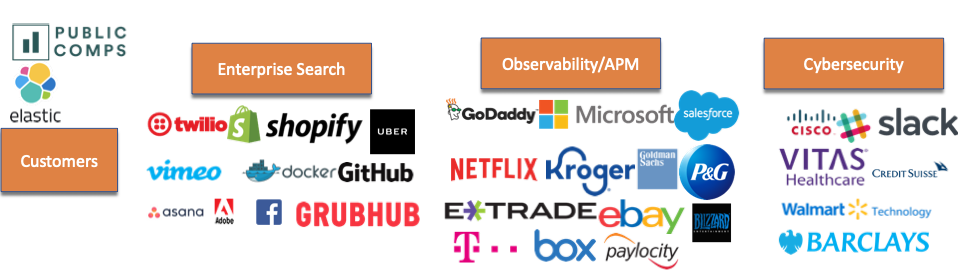
\includegraphics[width=\linewidth]{Assets/customers.png}
            \caption{نمونه‌های کابربردهای مختلف و مشتری‌ها\footnote{تصویر از \cite{publiccomps}}}
        \end{figure}
    
    \end{frame}

    \begin{frame}
        \frametitle{مفاهیم اولیه‌ی الستیک‌سرچ}
        \framesubtitle{آشنایی با اجزا}
    
        \begin{itemize}
            \item خوشه یا \lr{Cluster} \textcolor{whaleblue}{$\Leftarrow$} تعدادی از سرورهای الستیک‌سرچ که به هم متصل هستند
            \item گره یا \lr{Node} \textcolor{whaleblue}{$\Leftarrow$} هر یک از سرورهای الستیک‌سرچ در \lr{Cluster}
            \item سند یا \lr{Document} \textcolor{whaleblue}{$\Leftarrow$} هر یک از اسناد متنی که بارگذاری می‌شود
            \item مخزن یا \lr{Index} \textcolor{whaleblue}{$\Leftarrow$} مخازنی که دارای تعدادی سند با قالب یکسان هستند
            \item نگاشت یا \lr{Mapping} \textcolor{whaleblue}{$\Leftarrow$} قالب هر \lr{Index}
            \item تکه داده یا \lr{Shard} \textcolor{whaleblue}{$\Leftarrow$} هر \lr{Index} تعدادی \lr{Shard} دارد
            \item بخش یا \lr{Segment} \textcolor{whaleblue}{$\Leftarrow$} هر \lr{Shard} تعداد \lr{Segment} دارد
        \end{itemize}
    
    \end{frame}

    \begin{frame}
        \frametitle{مفاهیم اولیه‌ی الستیک‌سرچ}
        \framesubtitle{مقایسه با دیتابیس‌های رابطه‌ای}
    
        \begin{columns}
            \column{0.5\textwidth}
            \begin{block}{کمی نکات منفی در مورد الستیک!}
                \begin{itemize}
                    \raggedright
                    \item مفهوم \lr{Transaction} ندارد
                    \item پشتیبانی محدودتر از \lr{Join} 
                \end{itemize}
            \end{block}
            \begin{block}{نکته مهم}
                این محدودیت‌ها برای دیتابیس‌های 
                \lr{NoSQL} 
                و 
                \lr{Distributed}
                قابل انتظار است.
            \end{block}
            \column{0.5\textwidth}
            \begin{center}
                \begin{tabular}{|c|c|}
                    \hline
                    \rowcolor{whaleblue}
                    \textbf{\textcolor{white}{الستیک‌سرچ}} & \textbf{\textcolor{white}{دیتابیس‌های رابطه‌ای}} \\
                    \hline
                    \hline
                    \lr{Index} & \lr{Database} \\
                    \hline
                    \lr{Type\LTRfootnote{Removed since version 6.00}} & \lr{Table} \\
                    \hline
                    \lr{Document} & \lr{Row} \\
                    \hline
                    \lr{Field} & \lr{Column} \\
                    \hline
                    \lr{Mapping} & \lr{Schema} \\
                    \hline
                \end{tabular}
            \end{center}
        \end{columns}
            
    \end{frame}

    \begin{frame}
        \frametitle{کارایی در عملیات مختلف}
        \framesubtitle{جزئیات تست انجام شده}

        \begin{itemize}
            \item داده بارگذاری شده اطلاعات املاک تهران موجود در دیوار است. \cite{kaggle-dataset}
            \item این داده شامل 372332 رکورد و حجم خام \lr{143 MB} است.
            \item تست‌ها بر روی یک کامپیوتر شخصی با رم \lr{8 GB} و پردازنده \lr{Core i7-8550} انجام شده است.
        \end{itemize}
        
        \begin{alertblock}{ابزارهای مورد استفاده}
            برای کوئری زدن به الستیک از ابزار \lr{Kibana} که یک وب اپلیکیشن است استفاده شده است. 
            همچنین برای بارگذاری داده در الستیک با استفاده از ابزار \lr{Curl} درخواست \lr{HTTP} فرستاده شده است. 
            برای ارتباط با \lr{SQLServer} از \lr{Azure Data Studio} استفاده شده است.
        \end{alertblock}
    
    \end{frame}
    
    \begin{frame}
        \frametitle{کارایی در عملیات مختلف}
        \framesubtitle{عملیات ساختن مخزن}

        \centering
        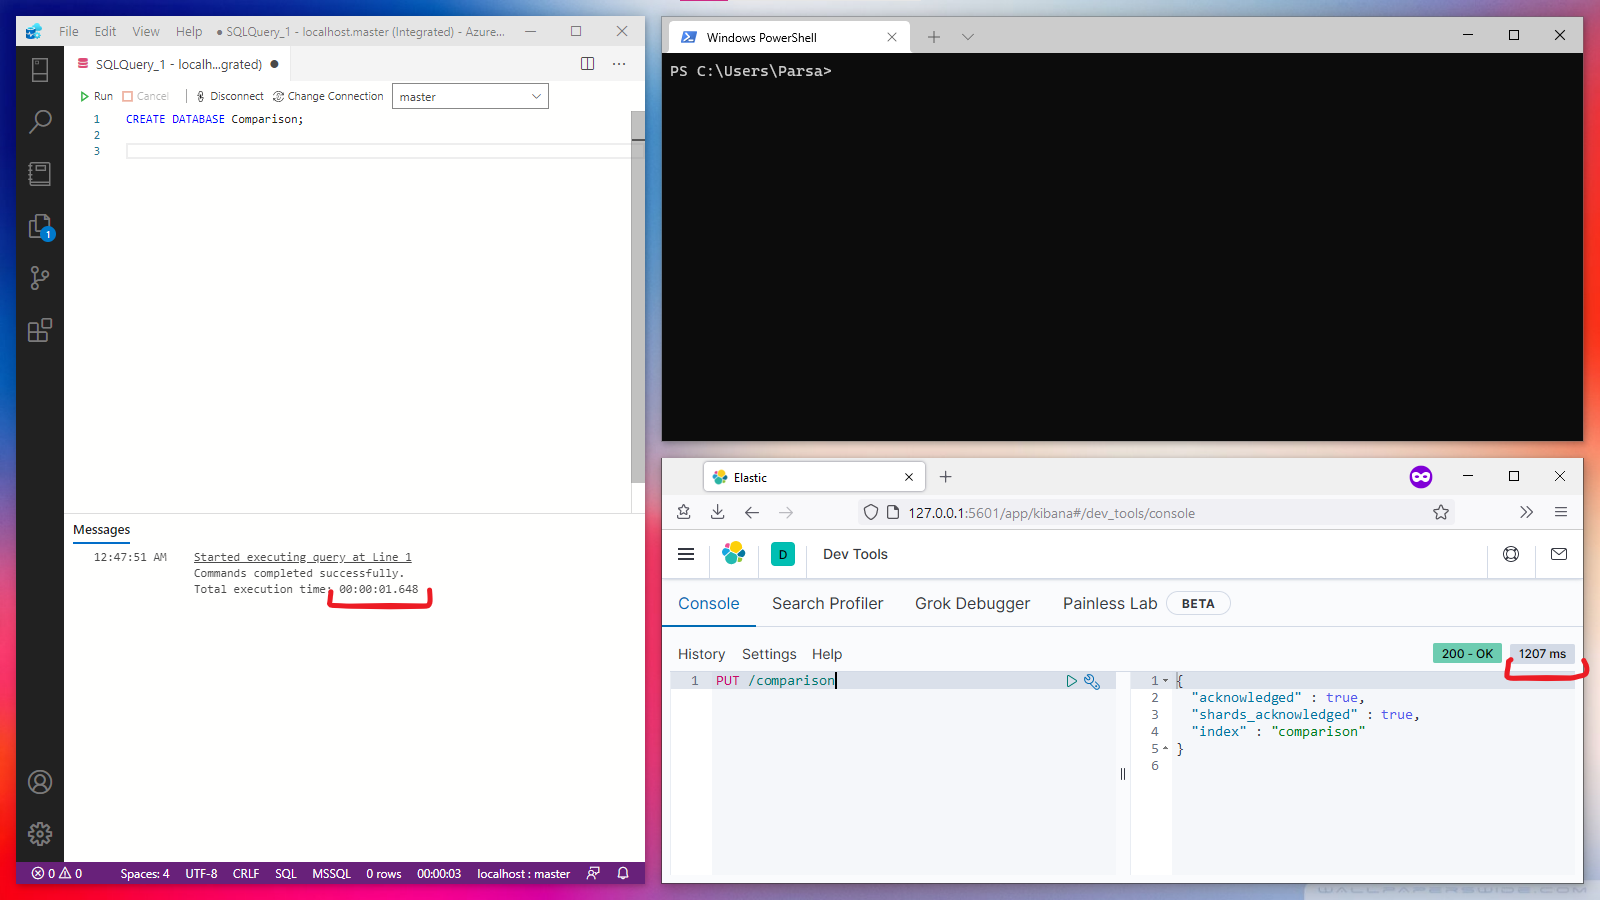
\includegraphics[width=0.9\linewidth]{Assets/PerformanceComparison/CreateIndex.png}
    
    \end{frame}
    
    \begin{frame}
        \frametitle{کارایی در عملیات مختلف}
        \framesubtitle{عملیات بارگذاری داده}

        \centering
        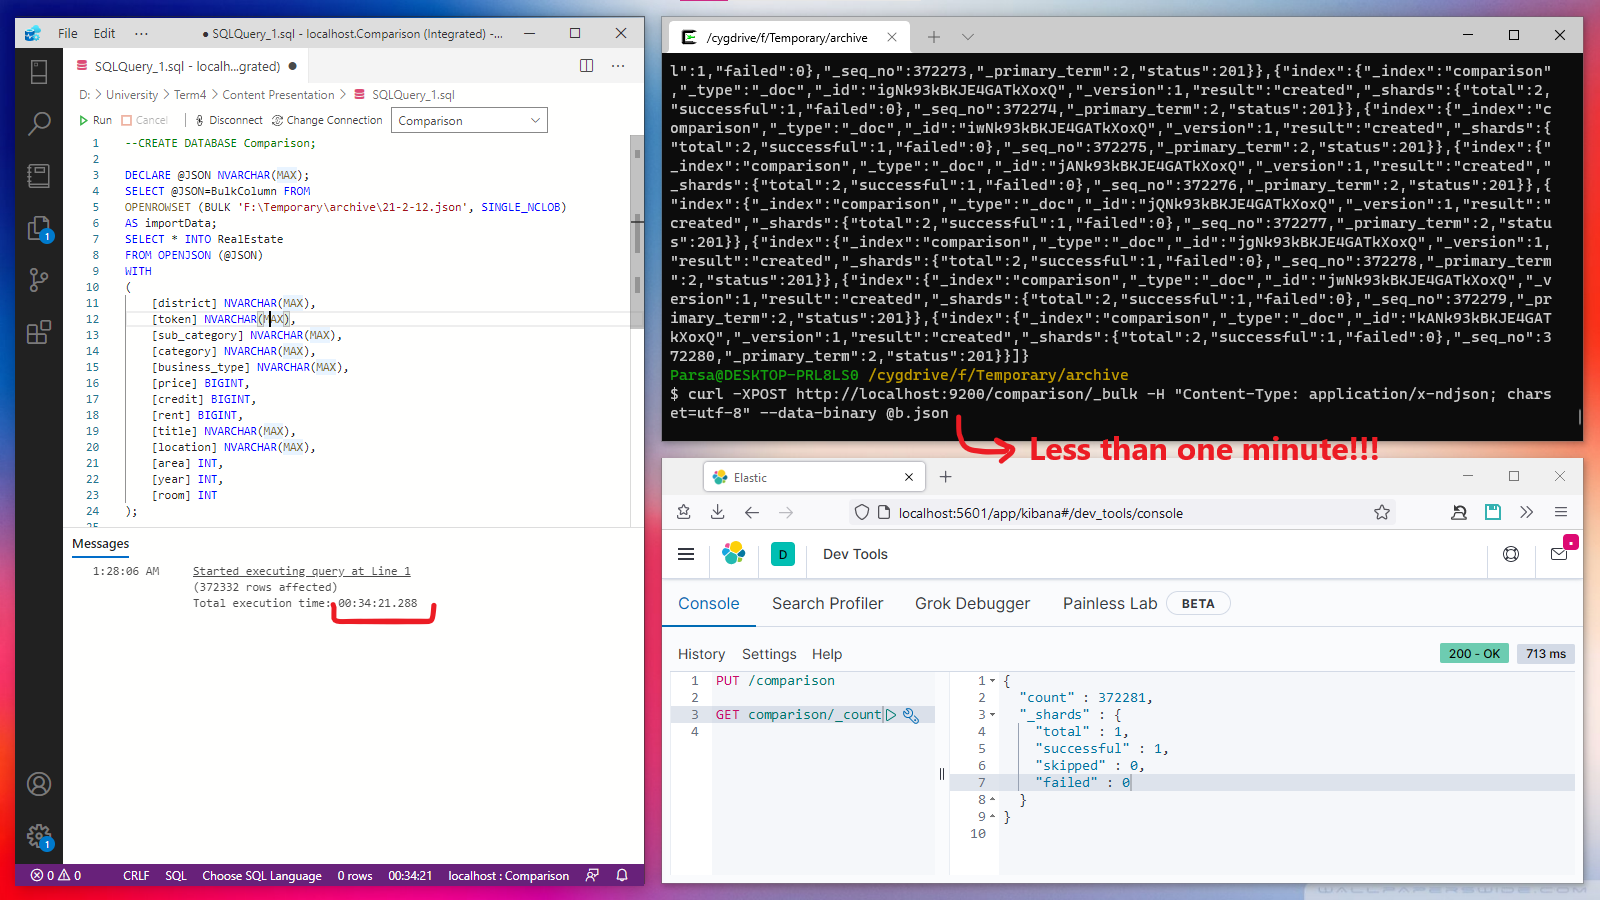
\includegraphics[width=0.9\linewidth]{Assets/PerformanceComparison/Bulk.png}
    
    \end{frame}
    
    \begin{frame}
        \frametitle{کارایی در عملیات مختلف}
        \framesubtitle{عملیات جستجو زیررشته}

        \centering
        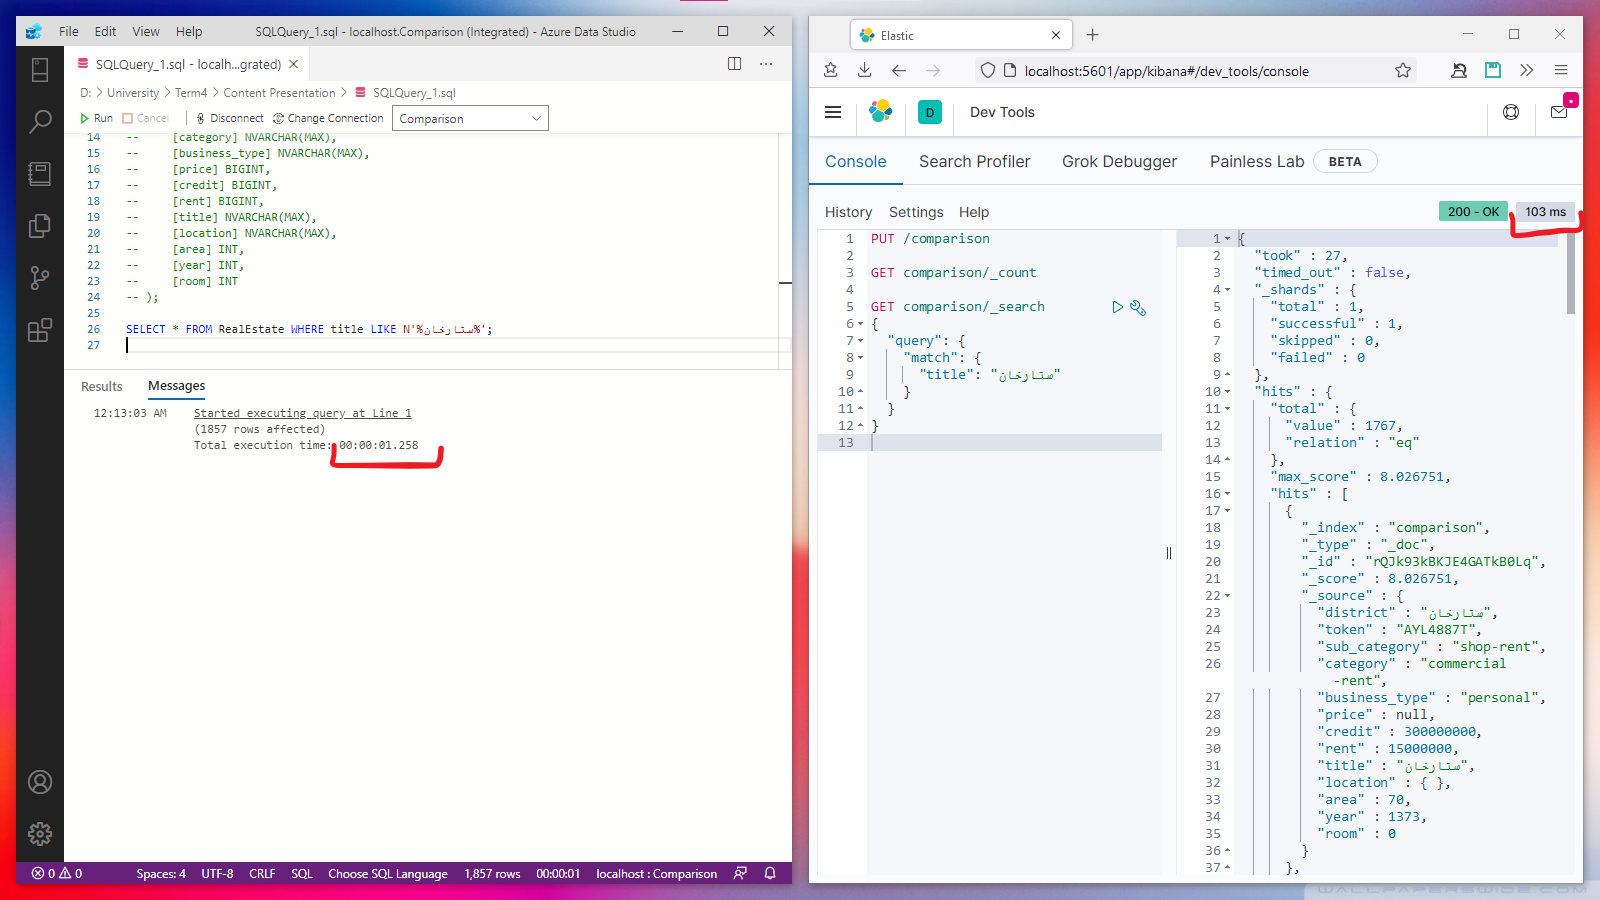
\includegraphics[width=0.9\linewidth]{Assets/PerformanceComparison/SearchWord.png}
    
    \end{frame}

    \begin{frame}
        \frametitle{کارایی در عملیات مختلف}
        \framesubtitle{عملیات جستجو بازه}

        \centering
        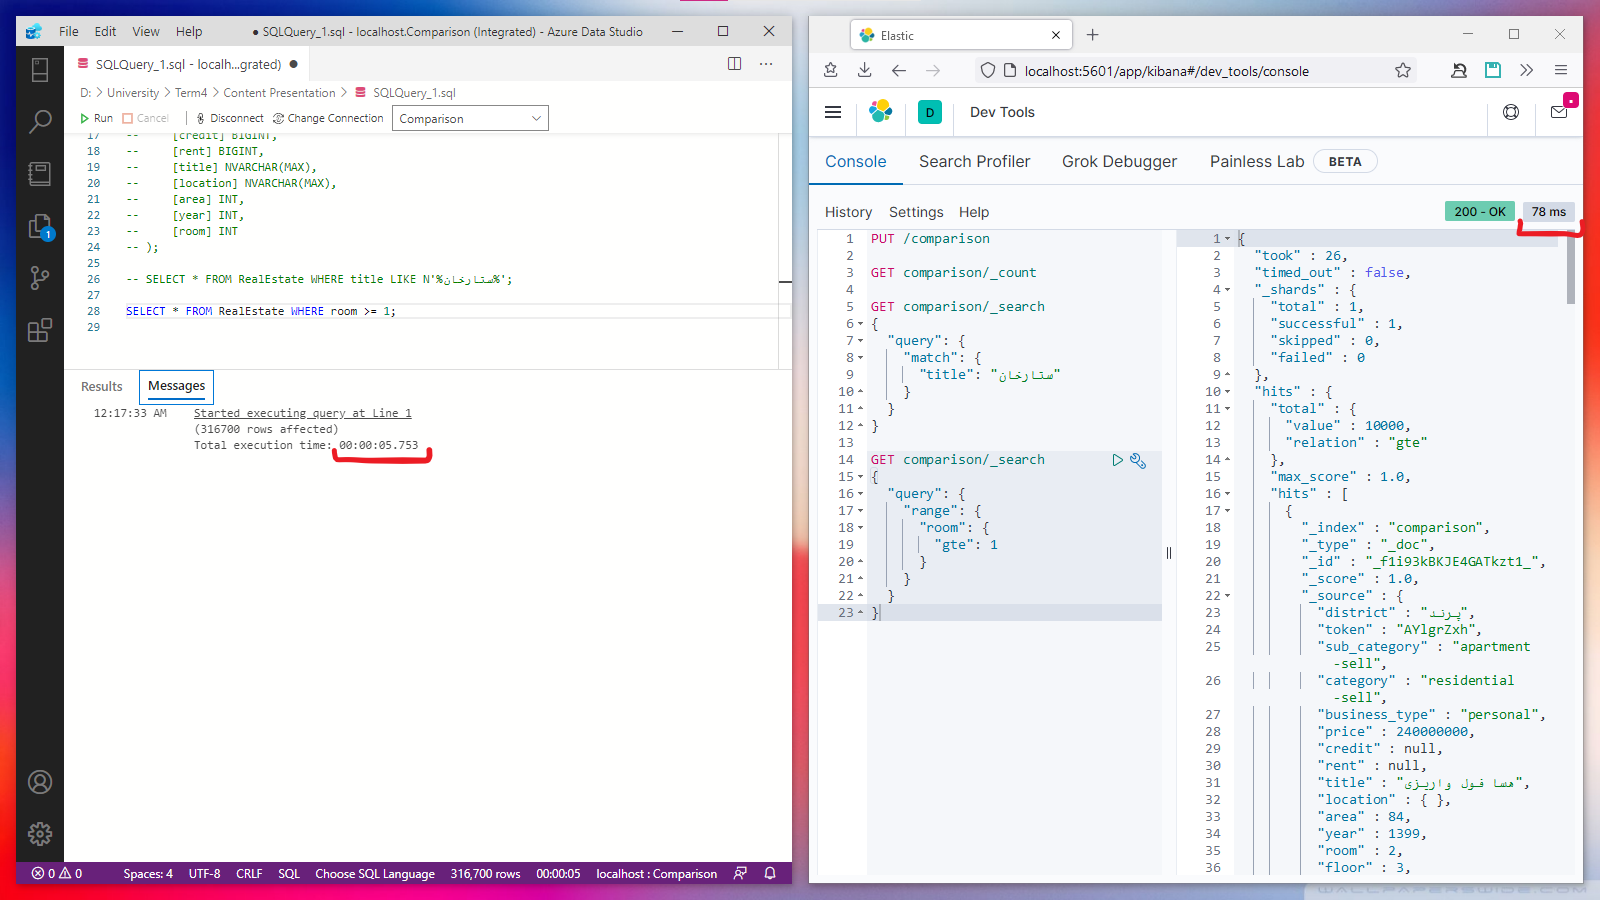
\includegraphics[width=0.9\linewidth]{Assets/PerformanceComparison/RangeSearch.png}
    
    \end{frame}

    \begin{frame}
        \frametitle{کارایی در عملیات مختلف}
        \framesubtitle{عملیات تجمعی (\lr{Aggregation})}

        \centering
        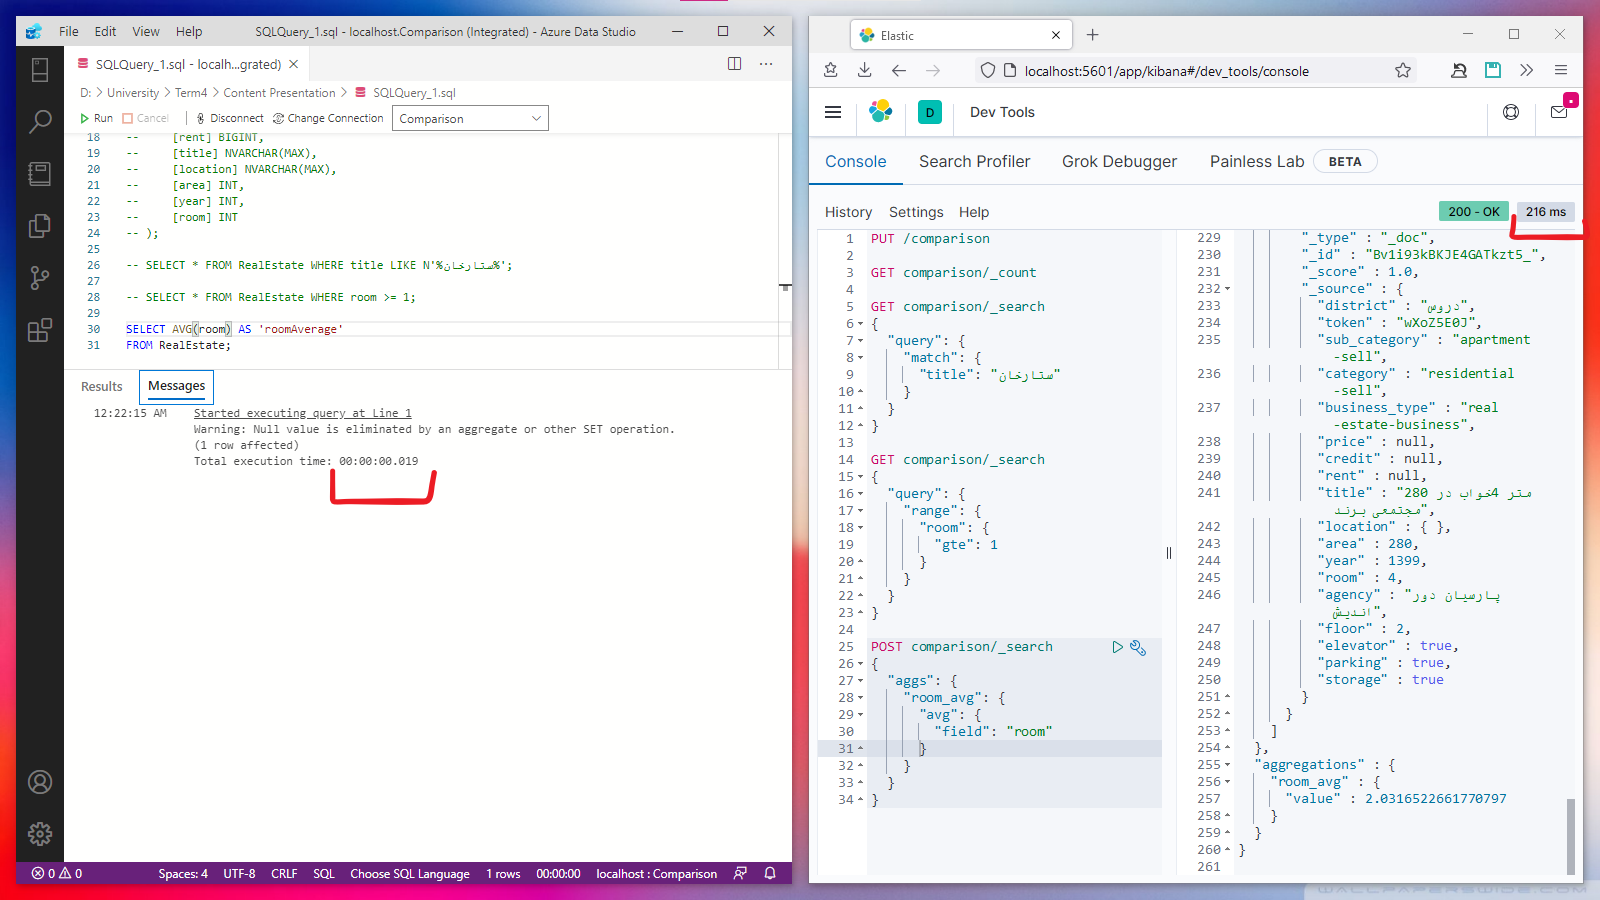
\includegraphics[width=0.9\linewidth]{Assets/PerformanceComparison/Aggregation.png}
    
    \end{frame}

    \begin{frame}
        \frametitle{کارایی در عملیات مختلف}
        \framesubtitle{عملیات تجمعی (\lr{Aggregation})}

        \centering
        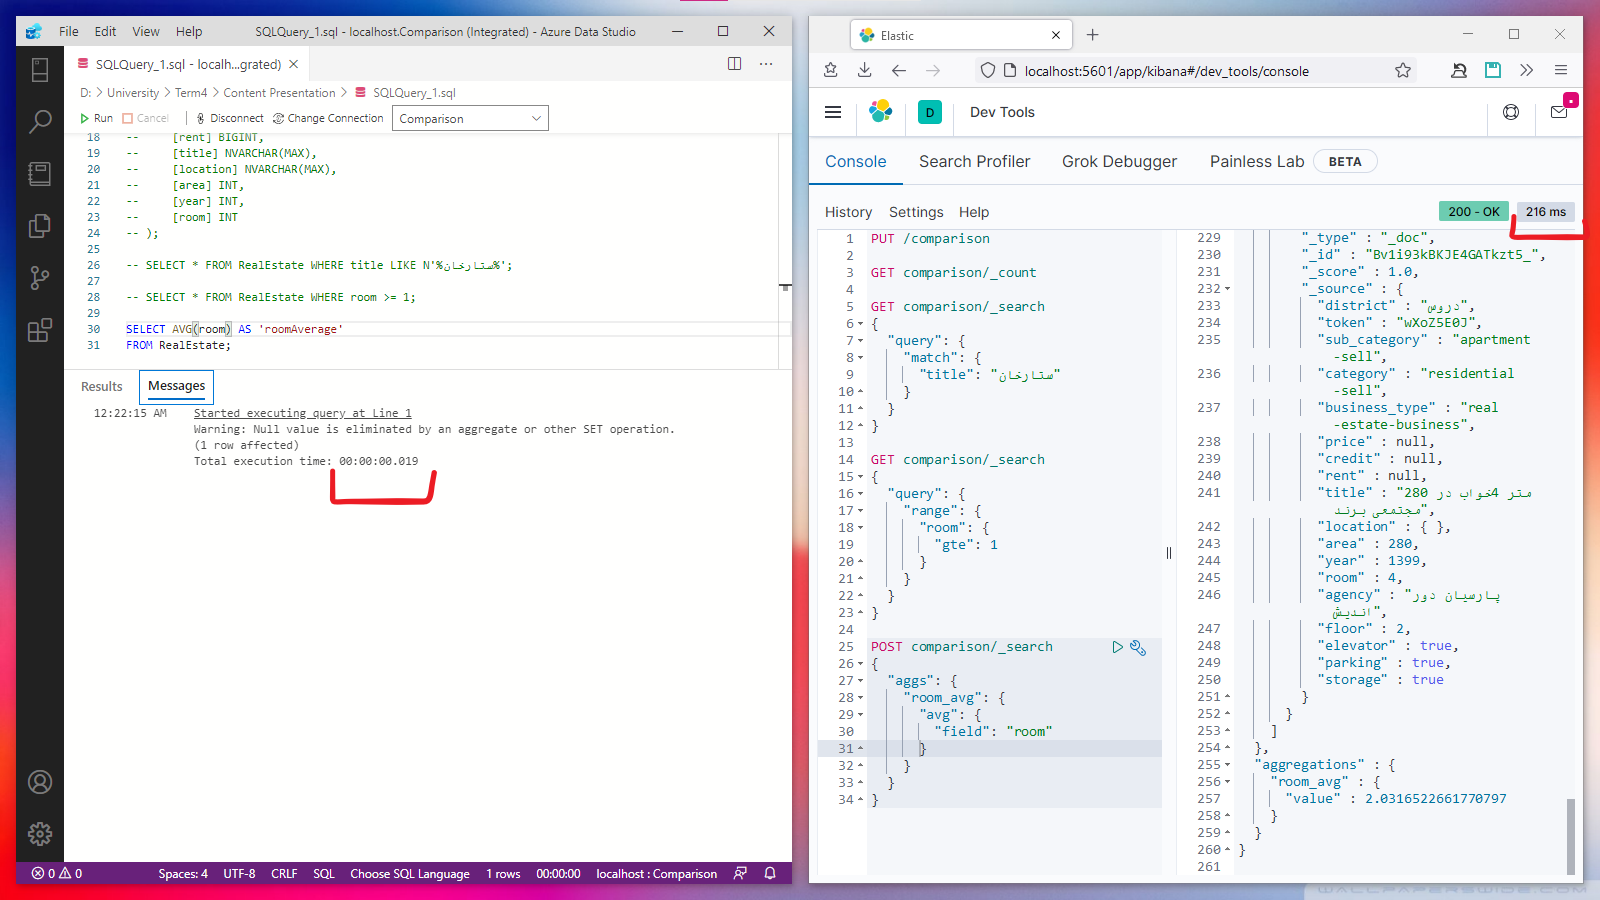
\includegraphics[width=0.9\linewidth]{Assets/PerformanceComparison/Aggregation.png}
    
    \end{frame}

    \begin{frame}
        \frametitle{الستیک‌سرچ کمی عمیق‌تر}
        \framesubtitle{\lr{Inverted index} در مقابل \lr{Index}}

        \begin{columns}
            \column{0.5\textwidth}
            سند1 : 
            \\
            سند2 :
            \column{0.5\textwidth}
            
        \end{columns}
    
    \end{frame}

    \begin{frame}
        \frametitle{منابع}

        \begin{latin}
            \printbibliography
        \end{latin}

        \tiny{اگر جایی منبع ذکر نشده از \cite{elastic-website} و \cite{definitive-guide} استفاده شده است.}
    
    \end{frame}
\end{document}